\documentclass[crop=false]{stdlocal}
\begin{document}
\section{Conclusions, Limitations, and Future Work} % (fold)
\label{sec:conclusions}

  During the course of this thesis, I build on the theory of \textcite{polthier2006} and formulated a rigorous mathematical foundation for the handling of discrete geodesics and curve smoothing algorithms on polyhedral surfaces.
  Hereby, special emphasis has been put on the consideration of boundaries which are often neglected by the general literature.
  Even on smooth manifolds, in the presence of boundaries the concept of locally shortest geodesics no longer agrees with the definition of straightest geodesics.
  This problem cannot be eliminated by simply redefining geodesic curvature on boundaries to be zero as this would lead to unintuitive results.
  State-of-the-art literature concerned with algorithms to generate geodesic paths and distances considers the concepts for discrete locally shortest and straightest geodesics as the de facto standard for the generalization of geodesics onto polyhedral surfaces.
  Regarding future work, I also want to consider other formulations of geodesics which may lead to a more intuitive interpretation and the removal of inconsistencies.

  % Following the mathematical foundation, different metrics for measuring the smoothness and similarity of curves have been proposed to allow for objective and quantitative comparisons of different curve smoothing states and techniques.
  % The largest problem is the uniform weighting along the length of a curve.
  % A curve moving with respect to its curvature gets much shorter at parts with a higher curvature value.
  % A general length mapping would be more intuitive.

  In the practical part of this work, I successfully designed and implemented various data structures to represent surface mesh curves as well as algorithmical primitives for their general movement and smoothing along polyhedral surfaces.
  All the implementation-specific details have been given as C++ code snippets to allow for reproducibility.
  The algorithmical primitives for smoothing surface mesh curves build on the work of \textcite{martinez2005} and \textcite{lawonn2014} by using data structures from \textcite{mancinelli2022}.
   % and a consistent curvature propagation.
  Additionally, the calculation of desired geodesic curvature values has been improved by using a weighted stencil of adjacent geodesic curvature values and applying it multiple times to geodesic curvatures of the initially given curve.
  % The main smoothing algorithm is based on an iterative approach to locally optimize geodesic curvature values in conjunction with surface-dependent penalty values to keep the outcome close to its original.
  The main smoothing algorithm is based on an iterative approach to locally optimize these geodesic curvature values.
  As such, it is part of the variational domain of solutions to curve smoothing.
  % This also allows for more general considerations such as anisotropic surface metrics.
  % Together with the defined smoothing metrics, I was able to proof that the algorithm indeed smoothes an initial curve and that it converges.

  % I have stated the concrete data structures for polyhedral surfaces and surface mesh curves and also added primitive operations.
  % This allowed for general construction on how to move a surface mesh curve along a polyhedral surface.
  % Also, I propose a more robust method for generating desired geodesic curvature values by using a weighting stencil.
  % Instead of an inconsistent curvature propagation, I have introduce curvature mapping.
  % The largest limitation of consistently moving surface mesh curves along polyhedral surface is the lack of mathematical convergence properties concerning discrete geodesic curvature.

  % The algorithms have been implemented as parallelized version on the CPU and GPU with the standard thread library of the C++ STL and the compute shaders of OpenGL, respectively.
  % I have designed tests based on the \citetitle{thingi10k} dataset to evaluate their robustness and efficiency.
  % Even for polyhedral surfaces consisting of millions of triangles, surface mesh curves exhibit typically only exhibit thousands of control points.
  % Most of curve smoothing or straightening algorithms are not parallelizable.
  % Due to iterative nature and the convergence behavior, I was able to show that CPU-based and GPU-based parallelization indeed allows for faster determination of smoothed curves.
  % Still, the smoothing of curves seems not to be the bottleneck of the application.
  % So, a parallelization for only a few thousands points might quickly become infeasible.
  % As there are data and flow dependencies in a curve smoothing procedure, parallelization is limited as it needs to constantly communicate with the CPU.
  % A bigger emphasis should lie on the robustness.

  As the movement of surface mesh curves depends on the topology of the polyhedral surface, the movement speed and convergence of algorithms can be slow for high-resolution surface meshes.
  Each iteration, a surface mesh curve may only propagate one vertex ahead.
  Especially for geodesics tracing, where the accumulated amount a curve may change is maximal, this process might be inefficient.
  Furthermore, the algorithmical primitives and smoothing procedure cannot considered to be robust if the polyhedral surface exhibits faces or vertices that are numerically extreme.
  Other methods, based on freely moving a curve in space followed by a projection onto the surface, could exhibit a better convergence rate and would not suffer from numerical instabilities originating from the surface mesh \autocite{crane2020}.

  Even for high-resolution polyhedral surfaces consisting of millions of triangles, surface mesh curves typically exhibit a few thousand control points.
  As such, the process of smoothing surface mesh curves does not appear to be the bottleneck of the overall program pipeline.
  Besides, most of the provided primitives for algorithms exhibit more complicated data and flow dependencies which hinder a parallelization on the CPU and GPU.
  As a result, the parallelization of the smoothing algorithm is expected to be unsuitable for general applications due to the high complexity of programming involved in comparison to the benefits of efficiency gain.
  Instead, future work should put serious focus on a robust implementation that would be able to handle many artificial and degenerate cases of polyhedral surfaces that often arise as smaller artifacts in real-world surface meshes.
  Such an implementation should be thoroughly tested by constructing generic tests that can be applied to a whole set of polyhedral surfaces such as the \citetitle{thingi10k} dataset \autocite{thingi10k,mancinelli2022}.
  % Apart from that, regarding the iterative nature of the main smoothing algorithm, a parallelization on the CPU could be realized by using a pipeline which

  Improving the iterative algorithm could be done by considering the funnel algorithm of \textcite{lee1984} that has been used by \textcite{mancinelli2022} to solve the discrete BVP for locally shortest geodesics in a finite amount of steps.
  To use the 2D funnel algorithm, \textcite{mancinelli2022} apply the geodesic unfolding to the whole triangle strip of a surface mesh curve at once and directly trace a straight line from the start to end of the strip.
  As the curvature-based unfolding primitive is a generalization of the geodesic unfolding, the funnel algorithm should also be applicable to the smoothing process based on desired geodesic curvatures as long as a solution exists.
  This could lead to an overall simplification and speed-up of the whole algorithm.
  However, future work would need to find a more general handling of the desired geodesic curvature.
  It would no longer be possible to append discrete values to already given control points and to let them propagate by an iterative approach to move the curve across the surface.
  Instead, one idea would be to offer a continuous geodesic curvature function and deducing discrete geodesic curvature values from it by integration.
  The mapping of values could be done with respect to the length of the curve.

  % For the implementation of curve smoothing inside a framework, further facilities should be provided.
  The smoothing of curves should be a process with emphasis on adaptivity and user controllability.
  In this sense, for an implementation of curve smoothing algorithms in more general frameworks, further facilities for the handling of fixed points would need to be added.
  If the desired geodesic curvature of a fixed control point is not constrained, the overall surface mesh curve can be viewed as two curves separated by this fixed point.
  In this case, both curve segments could be smoothed independently.
  The introduction of fixed control points with a constrained desired geodesic curvature, on the other hand, is not as simple.
  To handle such constraints, the curvature-based unfolding would also need to take adjacent geodesic curvatures into account.
  Unfortunately, the problematic behavior of discrete geodesic curvatures at the boundary, in this case, might forbid to choose fixed control points with a constrained desired geodesic curvature at the boundary of the surface.

  A framework incorporating surface mesh curves should also provide a sophisticated interface that allows a user to easily provide and manipulate initial curves.
  Hereby, constructing regular surface mesh curves from drawing lines on surfaces seems to be the most intuitive suggestion.
  To improve this process, future work should integrate the tracing of geodesics directly into the drawing of initial curves.
  In such a way, the generated surface mesh curve would mimic the trajectory provided by the user more closely.

  Regarding surface mesh artifacts, further basic requirements, such as the orientability or the fulfillment of vertex or edge manifold properties, are not given naturally by all surface meshes \autocite{thingi10k}.
  The violation of these constraints will most likely lead to program termination or other non-intuitive behavior.
  To build alternatives that are able to robustly cope with a large amount of different polyhedral surfaces, future work should take a look back at the basic data structures to represent surface mesh curves and adjacency information of polyhedral surfaces.
  The quad-edge algebra is an edge-based data structure to represent multiple adjacencies of a surface mesh in a versatile and efficient way.
  According to \textcite{guibas1985}, it encodes the graph and the dual graph of a surface mesh and was defined to also handle non-orientable or degenerate surface meshes whose faces may not solely consist of triangles.
  A quad-edge itself characterizes as a mixture of an edge and two adjacent faces at once and, consequently, should offer advantageous of both edge- and face-based data structures.
  As such, it seems to be an ideal candidate to provide simple, efficient, and robust representations for adjacencies and curves.
  On the other hand, quad-edge algebras are not as simple to generalize to higher dimensions as face-based data structures.

  Another problem that arises when dealing with general smoothing algorithms for surface mesh curves is the fact that smoothing itself is not a clear goal.
  There is no universally agreed-upon metric to measure the quality of a smoothing process.
  Implementing stopping criteria for algorithms or assigning desired geodesic curvature values are subjective processes and only provide heuristics to make an initially given curve intuitively smoother.
  However, for a rigorous design of smoothing, future work should involve the research on the generalization of norms that complete the spaces of $\mathrm{C^k}$-curves.
  Not only taking the maximum, average, or mean-squared geodesic curvature into account but also the values of its first or second derivative could allow to construct improved algorithms whose smoothing capabilities are provable.
  Also the proof of convergence for alternative smoothing algorithms, as it was done by \textcite{lawonn2014}, should be part of future work.

  The primitives involved to smooth a curve on a polyhedral surface, in general, incorporate locally-shortest geodesic tracing steps.
  Consequently, these methods also inherently shorten a curve while smoothing it.
  For methods that are solely based on geodesic curvature, this property is in general not true.
  For example, the reduction of geodesic curvature of a circle on the sphere must lead to a bigger circle and eventually converge to a great circle of the sphere.
  Indeed, with the use of the desired curvature stencil and a scaling parameter that is bigger or equal $1$, the length of the smoothing algorithm's result does not deviate too much from the original and might even be larger.
  Still, using the contraction property of the geodesics steps, is key to prove the existence of a solution and the convergence of the algorithm \autocite{martinez2005,lawonn2014}.
  For smoothing curves by expansion, future work should involve research to find the essential requirements that characterize the existence of an expanded curve.
  Please note, that this also includes properties of the underlying surface.
  Whereas in Euclidean space an expansion of a curve should always exist, in general surfaces this property is not fulfilled.

  The smoothing algorithm of \textcite{lawonn2014} wants to guarantee that the resulting curve is close to its original.
  It does this by using a distance envelope which suddenly forbids a moving curve to proceed at points that are too far away from the initial curve.
  Mathematically, this uncontinuous constraint transforms the underlying polyhedral surface into a smaller polyhedral surface with boundary.
  As for boundary vertices, it is not straightforward to use geodesic curvatures, only the curve shortening approach is applicable at these points.
  Unfortunately, this shortening approach does not reliably lead to a smoother curve.
  Instead, strong corners in the resulting curve might originate if the distance envelope is too small.

  \paragraph{Smoothing of Surface Mesh Curves by Using Geodesics and Scalar Potentials}\hfill\\
  Taking into account all the previous considerations, in the following, I am proposing an alternative algorithm for future work to generate smoothed surface mesh curves that need to be close to its original.
  Instead of using curvature-based transformations that may fail to be applied at boundary points, this algorithm would only use the generation of discrete locally shortest geodesics as its main primitive.
  Hereby, its main idea is based on the generalizations of distance envelopes to scalar potentials, that are used as penalty functions, and the following observation that figure~\ref{fig:lifting} schematically visualizes.
  Geodesics in the flat Euclidean plane as shown in figure~\ref{fig:lifting-flat} are given by straight lines.
  Thinking of plotting a 2D scalar potential over the Euclidean plane as it is given in figure~\ref{fig:lifting-lifted}, the graph of the scalar potential is no longer a surface embedded in 2D space but has been lifted and is now embedded in the 3D Euclidean space.
  As a direct consequence, locally shortest geodesics of the surface in figure~\ref{fig:lifting-lifted} are, in general, no longer straight lines.
  The trajectories of geodesics connecting two opposite points are forced to move around the bump in the middle, just like rivers need to move around a chain of mountains.

  \begin{figure}
    \centering
    \begin{subfigure}[c]{0.4\linewidth}
      \centering
      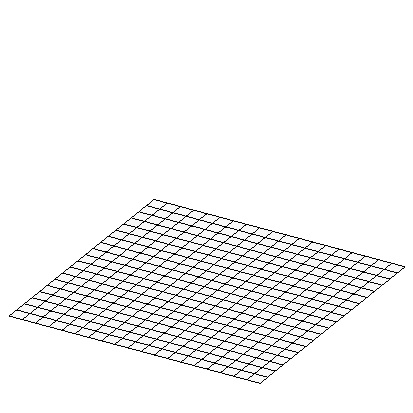
\includegraphics[width=\linewidth,trim={0mm 0 0 60},clip]{plots/plane.pdf}
      \caption{Flat in 2D with no Potential}
      \label{fig:lifting-flat}
    \end{subfigure}
    \hfill
    $\longrightarrow$
    \hfill
    \begin{subfigure}[c]{0.4\linewidth}
      \centering
      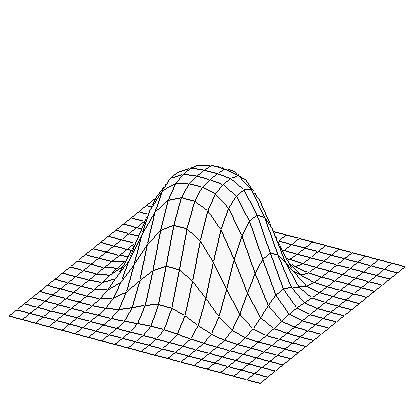
\includegraphics[width=\linewidth,trim={0mm 0 0 60},clip]{plots/gauss.pdf}
      \caption{Lifted to 3D with Potential}
      \label{fig:lifting-lifted}
    \end{subfigure}
    \caption[Lifting of Polyhedral Surfaces by Using Scalar Potentials]{%
      \textbf{Lifting of Polyhedral Surfaces by Using Scalar Potentials}\\
      The left images shows a bounded approximation of the 2D Euclidean plane by a polyhedral surface.
      As it can be seen on the right, constructing the graph of a scalar potential over this surface, leads to a lifting and an embedding in 3D Euclidean space.
      The geodesics for the lifted surface are no longer straight lines and will adapt to the form of the potential, just like a river does near a chain of mountains.
    }
    \label{fig:lifting}
  \end{figure}

  Constructing a scalar potential around an initially given curve, that penalizes farther distances with a higher potential value, the geodesics of its lifted surface embedded in 3D space when projected back onto the 2D plane should be smoothed curves that are close to the initial curve because the scalar potential was defined to fulfill this condition.
  This whole procedure can be generalized to 2D topological manifolds embedded in 3D Euclidean space.
  Using a scalar potential over such a surface, the graph of this potential is lifted into four dimensions and will describe a 2D topological manifold embedded in 4D Euclidean space.
  At this point, determining the geodesic on the lifted surface followed by a projection back onto the original surface would also lead to a smoothed curve which is close to its original.

  This method is not bound to use an iterative method but can make use of nearly all available algorithms for tracing geodesics or generating geodesic distance fields and may benefit from their robust and versatile implementation alternatives that have been found over the years.
  When given a scalar potential, this method always computes a clear goal which can be reached in finitely many steps \autocite{mancinelli2022,sharp2020}.
  Looking at it this way, this already proves the convergence of the algorithm as long as the geodesic primitive converges.
  By varying the potential, not only the smoothing of curves but also their general trajectory can be adaptively controlled by the user.
  To cope with existence of boundaries, scalar potentials could use very large values near the boundaries to push curves away and therefore prevent the appearance of strong corners.
  As the moving curve should never be too far away from its original, the scalar potential would not even need to be evaluated for the whole surface mesh but only for vertices near to the current curve by using a dynamic programming paradigm.
  The algorithm would benefit from the design and implementation of the algorithmical primitives given in this thesis.

  % Alternative Smoothing Algorithms: Your algorithm to lift the polyhedral surface into four dimensions by adding a scalar potential for geodesics.
  % Distance envelope is hard cut.
  % Keeping the distance small to the original curve can be done by your new method.

  % Anisotropic Metrics

  % Application to medicine

% section conclusions (end)
\end{document}
